\documentclass{article}
\usepackage{amsmath}
\usepackage{xstring}
\usepackage{catchfile}
\usepackage{graphicx}
\graphicspath{ {../octave/} }
\usepackage{url}
\usepackage{tikz}
\usepackage{tkz-euclide}

\CatchFileDef{\headfull}{../.git/HEAD}{}
\StrGobbleRight{\headfull}{1}[\head]
\StrBehind[2]{\head}{/}[\branch]
\IfFileExists{../.git/refs/heads/\branch}{%
    \CatchFileDef{\commit}{../.git/refs/heads/\branch}{}}{%
    \newcommand{\commit}{\dots~(in \emph{packed-refs})}}
\newcommand{\gitrevision}{%
  \StrLeft{\commit}{7}%
}

\title{Codec 2 Rate K Resampler}
\author{David Rowe\\ \\ Revision: {\gitrevision} on branch: {\branch}}
\date{\today}
\begin{document}

\maketitle

\section{Introduction}

To efficiently transmit spectral amplitude information Codec 2 700C uses a set of algorithms collectively denoted \url{newamp1}. One of these algorithms is the Rate K resampler which transforms the variable length vectors of spectral amplitude samples to fixed length $K$ vectors suitable for vector quantisation.  This document was written in order to explore and possibly improve rate $K$ resampling.

\section{Theoretical Model}

Consider a vector $\mathbf{a}$ of $L$ spectral amplitudes, sampled at time $t=nT$ seconds, where $n$ is the frame number, and $T$ is the frame period, typically $T=0.01$ seconds. 
\begin{equation}
\mathbf{a} = \begin{bmatrix} A_1, A_2, \ldots A_L \end{bmatrix} 
\end{equation}
$A_m$ is sampled at the frequency $f_m=mF0$ Hz for $m=1 \ldots L$, where $F0$ is the fundamental frequency (pitch) in Hz of the current frame, and $L$ is given by:

\begin{equation}
L=\left \lfloor \frac{F_s}{2F0} \right \rfloor
\end{equation}
$F0$ and $L$ are time varying as the pitch track evolves over time. For speech sampled at $F_s=8$ kHz $F0$ is typically in the range of 50 to 400 Hz, giving $L$ in the range of 10 $\ldots$ 80. \\

To quantise and transmit $\mathbf{a}$, it is convenient to resample $\mathbf{a}$ to a fixed length $K$ element vector $\mathbf{b}$ using a resampling function:
\begin{equation}
\begin{split}
\mathbf{y} &= \begin{bmatrix} Y_1, Y_2, \ldots Y_L \end{bmatrix} = H(\mathbf{a}) \\
\mathbf{b} &= \begin{bmatrix} B_1, B_2, \ldots B_K \end{bmatrix} = R(\mathbf{y})
\end{split}
\end{equation}
Where $H()$ is a filter function chosen to smooth the spectral amplitude samples $A_m$ while not significantly altering the perceptual quality of the speech; and $R()$ is a resampling function. To model the logarithmic frequency response of the human ear $B_k$  are sampled on $K$ non-linearly spaced points on the frequency axis:
\begin{equation}
\begin{split}
f_k &= warp(k,K) \ \textrm{Hz} \quad k=1 \ldots K \\
warp(1,K) &= 200 \ \textrm{Hz} \\
warp(K,K) &= 3700 \ \textrm{Hz}
\end{split}
\end{equation}
where $warp()$ is a frequency warping function. Codec 2 700C uses $K=20$, and $warp()$ is defined using the Mel function (Figure \ref{fig:mel_fhz}) which samples the spectrum more densely at low frequencies, and less densely at high frequencies:
\begin{equation} \label{eq:mel_f}
mel(f) = 2595log_{10}(1+f/700)
\end{equation}
The inverse mapping of $f$ in Hz from $mel(f)$ is given by:
\begin{equation} \label{eq:f_mel}
f = mel^{-1}(x) = 700(10^{x/2595} - 1);
\end{equation}

\begin{figure}[h]
\caption{Mel function}
\label{fig:mel_fhz}
\begin{center}
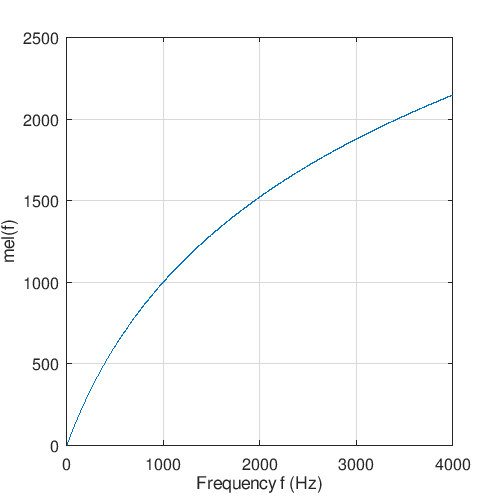
\includegraphics[width=8cm]{ratek_mel_fhz}
\end{center}
\end{figure}

We wish to use $mel(f)$ to construct $warp(k,K)$, such that there are $K$ evenly spaced points on the $mel(f)$ axis (Figure \ref{fig:mel_k}).  Solving for the equation of a straight line we can obtain $mel(f)$ as a function of $k$, and hence $warp(k,K)$ (Figure \ref{fig:warp_fhz_k}):
\begin{equation} \label{eq:mel_k}
\begin{split}
g &= \frac{mel(3700)-mel(200)}{K-1} \\
mel(f) &= g(k-1) + mel(200)
\end{split}
\end{equation}
Substituting (\ref{eq:f_mel}) into the LHS:
\begin{equation} \label{eq:warp}
\begin{split}
2595log_{10}(1+f/700) &= g(k-1) + mel(200) \\
f = warp(k,K) &= mel^{-1} ( g(k-1) + mel(200) ) \\
\end{split}
\end{equation}
and the inverse warp function:
\begin{equation} \label{warp_inv}
k = warp^{-1}(f,K) = \frac{mel(f)-mel(200)}{g} + 1
\end{equation}

\begin{figure}[h]
\caption{Linear mapping of $mel(f)$ to Rate $K$ sample index $k$}
\vspace{5mm}
\label{fig:mel_k}
\centering
\begin{tikzpicture}
\tkzDefPoint(1,1){A}
\tkzDefPoint(5,5){B}
\draw[thick] (1,1) node [right]{(1,mel(200))} -- (5,5) node [right]{(K,mel(3700))};
\draw[thick,->] (0,0) -- (6,0) node [below]{k};
\draw[thick,->] (0,0) -- (0,6) node [left]{mel(f)};
\foreach \n in {A,B}
  \node at (\n)[circle,fill,inner sep=1.5pt]{};
\end{tikzpicture}
\end{figure}

\begin{figure}[h]
\caption{$warp(k,K)$ function for $K=20$}
\label{fig:warp_fhz_k}
\begin{center}
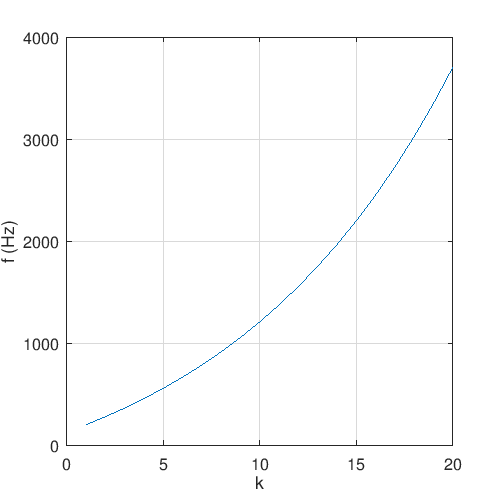
\includegraphics[width=8cm]{warp_fhz_k}
\end{center}
\end{figure}

The rate $K$ vector $\mathbf{b}$ is vector quantised for transmission over the channel:
\begin{equation}
\hat{\mathbf{b}} = Q(\mathbf{b})
\end{equation}
The rate filtered rate $L$ vector can then be recovered by resampling $\mathbf{\hat{b}}$ using another resampling function:
\begin{equation}
\hat{\mathbf{y}} = S(\hat{\mathbf{b}})
\end{equation}
A useful error metric is the mean square error:
\begin{equation} \label{eq:E1}
\begin{split}
E & =\frac{1}{L_{max}-L_{min}+1}\sum_{m=L_{min}}^{L_{max}}(Y_m-\hat{Y}_m)^2 \\
L_{min} & = round(200/F0) \\
L_{max} & =\left \lfloor 3700/F0  \right \rfloor
\end{split}
\end{equation}
In the case where there is no filtering (e.g. \url{newamp1}) then:
\begin{equation}
\begin{split}
H(\mathbf{x}) &= \mathbf{x} \\
\mathbf{y} &= \mathbf{a} \\
\hat{\mathbf{a}} &= \hat{\mathbf{y}} \\
E &=\frac{1}{L_{max}-L_{min}+1}\sum_{m=L_{min}}^{L_{max}}(A_m-\hat{A}_m)^2 
\end{split}
\end{equation}
If $A_m$ are in dB, $E$ can be denoted the spectral distortion in $dB^2$, which can be averaged over a testing database of $N$ frames to obtain mean spectral distortion.

Consider a choice of $warp()$ with linear (non-warped) sampling of the frequency axis, no filtering such that $H(\mathbf{x})=\mathbf{x}$, and an ideal quantiser $Q$ such that $\hat{\mathbf{b}} = \mathbf{b}$. If $K<L$ information may be lost due to undersampling, which implies $\hat{\mathbf{a}} \neq \mathbf{a}$.  
With nonlinear sampling, there will be local undersampling where the sampling rate of $\mathbf{b}$ is less than that of $\mathbf{a}$:
\begin{equation} \label{eq:local_undersampling}
warp(k+1,K)-warp(k,K) < F0
\end{equation}
If $A_m$ is changing rapidly, undersampling may introduce undesirable aliasing, which may manifest as noise that is superimposed on $\mathbf{b}$. This noise may reduce perceptual quality and consume valuable quantiser bits for no benefit. Therefore $H()$ should be chosen to smooth high frequency detail such that local undersampling and uncontrolled aliasing is minimised. This may be restated as choosing $H()$ to minimise $E$ (\ref{eq:E1}) when $\hat{\mathbf{b}} = \mathbf{b}$.

\section{Suggested Experiments}
 
Here are a suggested set of experiments to evaluate the ideas presented in this document.  Some of them require informal listening tests, others have objective measures which could be used as the basis for automated tests:

\begin{enumerate}

\item The baseline resampling (currently a 2nd order polynomial) is a potential source of distortion.  Conduct an experiment to test the theory that $E$ is small (and perceptual quality high) for $K>L$ using linear frequency sampling, $H(\mathbf{x})=\mathbf{x}$ and large $K$.

\item How to demonstrate aliasing?  Well we can run current rate K code, that uses a 2nd order parabolic resampler.  Then compare with a "better" resampler that uses filtering.  Perform an informal listening test over a small set of samples.  Goal is to show reduced $E$ with similar perceptual quality.  Smoothing does reduce information so there will be a trade off.  Too much smoothing and perceptual quality will reduce.  We should also notice improved VQ performance, as we won't be quantising noise.

\item A useful property is sensitivity to quantisation, which could be defined as $\frac{\partial E}{\partial \mathbf{b}}$. For example, given a 1dB RMS error in the elements of $\mathbf{b}$, what is the impact on $E$?

\item To minimise bit rate, it is common to transmit $\mathbf{b}$ to the receiver at period $T/D$ seconds, where $D$ is the decimation ratio, and discarding the intermediate $D-1$ frames. A useful property is the ability to smoothly interpolate between transmitted frames $\mathbf{b}_n$ and $\mathbf{b}_{n+D}$ to recover $\mathbf{b}_{n+i}$ where $i=1 \ldots D-1$.  Need a definition for smoothness.

\item Speech evolves slowly over time compared to the $T=0.01$ second frame period.  Adjacent frames of speech parameters such as $\mathbf{a}_n$ and $\mathbf{a}_{n+1}$ have some correlation which can be used to obtain coding efficiency:
\begin{equation} \label{eq:delta}
\begin{split}
\mathbf{b}_{n+1} & = \mathbf{b}_{n} + \mathbf{\Delta}_n \\
\mathbf{\Delta}_{n+1} & = \mathbf{b}_{n+1} - \mathbf{b}_{n}
\end{split}
\end{equation}

In general $\mathbf{\Delta}_n$ can be encoded with less bits than $\mathbf{b}_n$.  However consider the case where there is significant noise due to undersampling:
\begin{equation}
\mathbf{\hat{b}}_n = \mathbf{b}_{n} + \mathbf{n}_{n}
\end{equation}
where $\mathbf{n}_{n}$ is a vector of noise samples with an unknown distribution. Substituting into (\ref{eq:delta}):
\begin{equation}
\mathbf{\Delta}_{n+1} = \mathbf{b}_{n+1} - \mathbf{b}_{n} + \mathbf{n}_{n+1} - \mathbf{n}_{n}
\end{equation}
If $\mathbf{n}_{n}$ and $\mathbf{n}_{n+1}$ are not well correlated they may become a significant source of noise that is summed with $\mathbf{\Delta}_{n}$, reducing the effectiveness of the quantister that will need to waste bits quantising the noise. We would therefore expect that in the absence of undersampling noise, delta coding in time should result in increased quantiser efficiency.

\item Small changes in $\mathbf{a}$ input should result in small changes in $\mathbf{b}$ indicating a lack of sensitivity and undersampling noise in $R$.  If $R$ is sensitive, we may notice VQ choices changing from frame to frame for stationary speech.

\item If the sample rate $K$ is sufficiently high (or bandwidth of $\mathbf{a}$ sufficiently constrained), the actual VQ dimension won't matter.  The decorrelation properties of the VQ will ensure it achieves the same distortion over a range of dimensions.  A large enough dimension $K$ could be chosen to simplify $S$, which could be linear resampling. It would be good to decouple $warp()$ from K.
\end{enumerate}

\section{Experiment 1: rate $K>L$ linear}

This experiment tests the ability to resample perfectly ($E=0$) with $K>L$, no filtering ($H(x)=x$) and linear frequency sampling and was implemented with Octave scripts \path{ratek1_fbf.m} and \path{ratek1_batch.m}.

Figure \ref{fig:ratek1_big_dog_50} illustrates why the resampler choice is important.  In the region of F1, the spectral samples $A_{m}$ are changing quickly.  The parabolic resampler fails to track these changes leading to distortion in a perceptually important feature of the spectrum.  When the resampler is viewed as a filter, this can be interpreted as a low pass response in the parabolic resampler, and is most noticable when $K$ is close to $L$.

\begin{figure}[h]
\caption{Frame 50 of big\_dog sample with $K=40$ just larger than $L=37$, 2nd order parabolic resampler.  Note distortion around F1 at 500 Hz }
\label{fig:ratek1_big_dog_50}
\begin{center}
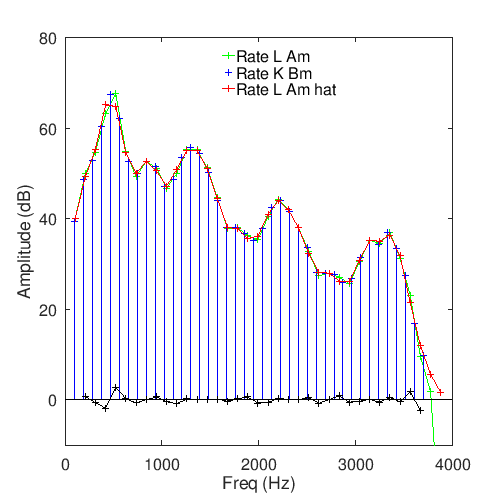
\includegraphics[width=10cm]{ratek1_big_dog_50}
\end{center}
\end{figure}

Figure \ref{fig:ratek1_hts_E} shows the spline and parabolic resampler $E$, plotted against $F0$ for a 24 second sample containing four speakers.  Table \ref{table:ratek1_mean_E} is the mean spectral distortion $E$ over the sample.  The spline interpolator perfoms better than the parabolic interpolator.  $L$ is time varying, but as it approaches $K$, $E$ increases, once again showing that interpolators struggle with $K$ close to $L$.

\begin{table}[h]
\centering
\begin{tabular}{c c }
 \hline
 Resampler & mean $E$ $dB^2$ \\
 \hline
 spline & 0.02 \\ 
 para  & 0.31 \\
 \hline
\end{tabular}
\caption{Table to test captions and labels.}
\label{table:ratek1_mean_E}
\end{table}

In this experiment with $K=80$ both resamplers have low average $E$ (less than $1 dB^2$). On inspection using \url{ratek_fbf} the occasional high $E$ frames were found to be unvoiced speech or background noise, where the pitch estimator tends to return low $F0$ (high $L$) estimates.  Fortunately the ear is quite insensitive to spectral distortion in unvoiced of background noise frames, so it is unlikley these errors are audible.  However with a lower choice of $K$ we would start to get resampling distortion duing voiced speech as $K$ approaches $L$ (Figure \ref{fig:ratek1_big_dog_50}), or when $K<L$, aliasing.

\begin{figure}[h]
\caption{Scatter plot of $E$ versus $F0$ for \emph{hts} sample, spline and parabolic resampler}
\label{fig:ratek1_hts_E}
\begin{center}
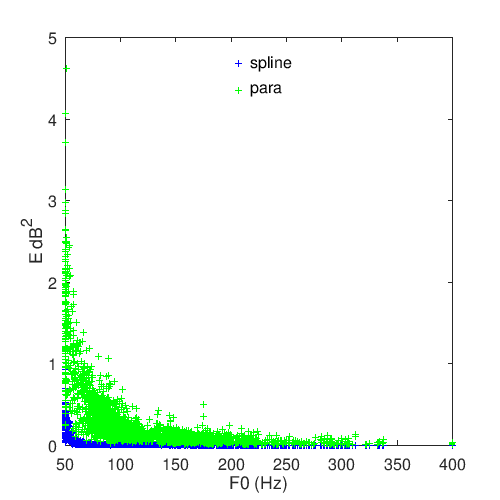
\includegraphics[width=8cm]{ratek1_hts_E.png}
\end{center}
\end{figure}

\begin{figure}[h]
\caption{Histogram of $E$ for spline and parabolic resampler}
\label{fig:ratek1_hts_hist}
\begin{center}
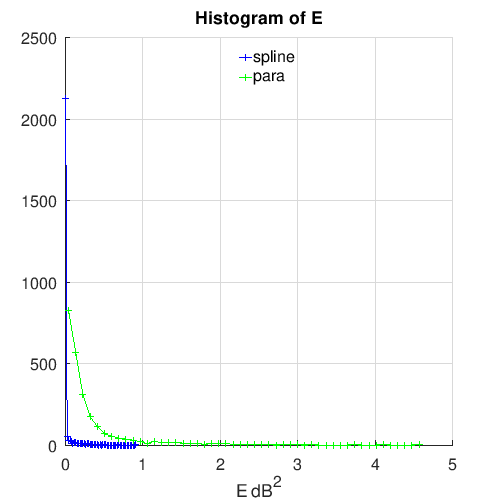
\includegraphics[width=8cm]{ratek1_hts_hist.png}
\end{center}
\end{figure}

Conclusions:
\begin{enumerate}
\item The resampler matters, especially when $K$ is close to $L$.  The current rate $K$ Codec 2 700C system uses $K < L$ (at least at high frequencies) with a parabolic resampler and no filtering.  This may be suffering from resampling noise that affects VQ performance and speech quality. It seems prudent to use a low distortion resampler.  We do not want to add any additional distortion sources to our system.

\item We intend to use $K<L$, which will lead to aliasing distortion.  It would be wise to filter $A_{m}$ prior to resampling to remove the possibility of aliasing and resampler distortion, that is choose $H()$ such that with $\mathbf{b}=\hat{\mathbf{b}}$, $E$ (\ref{eq:E1}) is minimised.

\item Once filtered, there will be some minimum value of $K_{min}$ required for $\mathbf{b}$ such that the rate $L$ vector $\hat{\mathbf{f}}$ can be recovered with minimal $E$. However we are free to choose $K>K_{min}$ as the "bandwidth" of the sampled sequence (and presumably VQ distortion for a given number of bits) will be independant of $K$ when $K>K_{min}$.  While a larger $K$ will use more VQ storage, it may simplify resampling at the receiver.  If $K$ is large enough, a simple linear resampler may suffice.

\item With non-linear frequency sampling, we may need a high local rate near F1 to accurately represent sharp formants, especially for males.  There may be other ways to encode this information, for a example a resampling function or VQ that takes into account $F0$ - "sharpening" F1 for low $F0$ speakers.

\item The newamp1 postfilter is an experimentally derived algorithm that raises peaks and lowers troughs in the rate $K$ spectrum, effectively "sharpening" formants.  When used after vector quantisation it has a large impact on Codec 2 700C speech quality, especially for male speakers.  However it's function is not well understood and in some cases it may be adding distortion.  The sensitivity of F1 to low $K$ resampling provides some hints as to why the postfilter is required.  Resampler distortion in Figure \ref{fig:ratek1_big_dog_50} distorts F1, which is further degraded by vector quantisation.  An increased sample rate and better resampling may reduce the need for the postfilter.

\end{enumerate}

\section{Experiment 2 - Filtering}

The goal of this experiment is to filter the spectral amplitudes $\mathbf{a}$ such that they can be more coarsely resampled without resampling or aliasing errors, and with mimimal impact on the perceptual quality.
The $m$th filtered sample can be obtained by:
\begin{equation}
Y_m = \sum_{k=st}^{en}A_k h(k)
\end{equation}
where $h(k)$ is sequence of samples defining a suitable filter, and $st$ and $en$ define the start and end harmonics used as input to the filtering operation for the $m$th sample.

As we wish to resample on a non-linear frequency axis, we need a set of filters that become wider as frequency increases. We can use the frequency warping function to divide the speech spectrum into $N_b$ bands, with the centre frequency of each band given by:
\begin{equation}
\begin{split}
f_b &= warp(b,N_b) \ \textrm{Hz} \quad b=1 \ldots N_b \\
warp(1,Nb) &= 200 \ \textrm{Hz} \\
warp(Nb,Nb) &= 3700 \ \textrm{Hz}
\end{split}
\end{equation}
For this experiment, we wish to separate the filtering $H()$ from the rate $K$ resampling operation, and perform the filtering on the rate $L$ samples $A_m$.  In this case it is convenient to treat $b$ as a continuous variable.  Given the $m$th harmonic, we can determine the filter band:
\begin{equation}
\begin{split}
f_b &= mF0 \\
b &= warp^{-1}(f_b,N_b) \\
\end{split}
\end{equation}
A common choice for filtering $g(k)$ is a triangular function, which tapers down to zero in the centre of adjacent bands $b-1$ and $b+1$.  This can be defined in terms of the harmonic indexes, as illustrated in  Figure \ref{fig:triangle_filter}.
\begin{equation}
\begin{split}
st &= max(1,round(warp(b-1,N_b)/F0)) \\
en &= min(L,round(warp(b+1,N_b)/F0)) \\
g(k) &= \frac{k-st}{m-st} \quad k=st \ldots m-1 \\
g(m) &= 1 \\
g(k) &= \frac{en-k}{en-m} \quad k=m+1 \ldots en \\
g_{sum} &= \sum_{k=st}^{en}g(k) \\
h(k) &= g(k)/g_{sum}
\end{split}
\end{equation}
Note the normalising term $g_{sum}$ to ensure the energy of $A_m$ is not altered by the filtering operation. Figure \ref{fig:filters_h} is an example set of filters. It can be seen that $N_b$ controls the filtering.  As $Nb$ becomes smaller, $g(k)$ becomes wider, reducing the rate of change of the filtered spectral samples $Y_m$.  While this presumably improves VQ performance, at some point it will also affect the perceptual quality of the speech.

\begin{figure}[h]
\caption{Triangular Filter $h(k)$.  Note asymmetry on linear frequency axis}
\vspace{5mm}
\label{fig:triangle_filter}
\centering
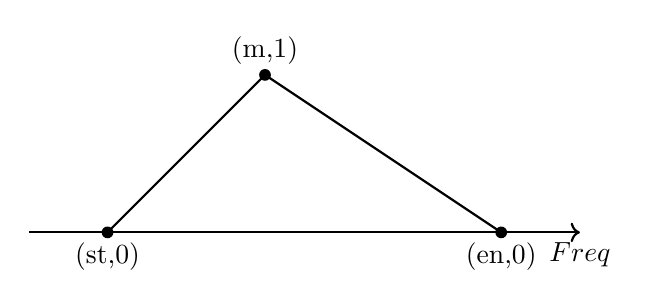
\begin{tikzpicture}
\tkzDefPoint(0,0){A}
\tkzDefPoint(2,2){B}
\tkzDefPoint(5,0){C}
\draw[thick] (0,0) node [below]{(st,0)} -- (2,2) node [above]{(m,1)};
\draw[thick] (2,2) -- (5,0) node [below]{(en,0)};
\draw[thick,->] (-1,0) -- (6,0) node [below]{$Freq$};
\foreach \n in {A,B,C}
  \node at (\n)[circle,fill,inner sep=1.5pt]{};
\end{tikzpicture}
\end{figure}

\begin{figure}[h]
\caption{Filters $h(k)$ for $N_b=10, m=1 \ldots L, F0=200 \textrm{Hz}, L=20$.  There is no smoothing (length 1 filters) up to 1000 Hz, higher frequencies have progressively more smoothing.}
\label{fig:filters_h}
\begin{center}
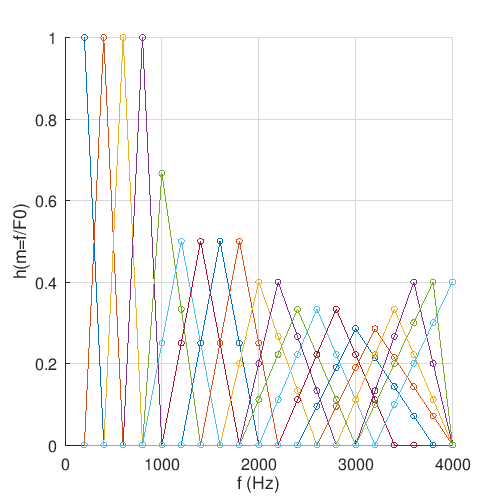
\includegraphics[width=8cm]{filters_h.png}
\end{center}
\end{figure}

Figure \ref{fig:ratek2_E_K_hts} illustrates the effect of varying $K$ for a family of filters by attempting to recover $\hat{\mathbf{y}} = S(R(\mathbf{y}))$ where $\mathbf{y}=H(\mathbf{a})$. As suggested in the conclusion of Experiment 1, once $K>K_{min}$, $\hat{\mathbf{y}}$ can be recovered with very low distortion $E$, even though $K<L$ for many frames.

As $N_b$ increases, the filter width reduces such that $h(k)=1$ for $k=m$ and $h(k)=0$ for $k\ne m$. Thus $N_b=100$ (where $N_b=100 > L_{max}$=80) corresponds to no filtering.  As expected, with $N_b=100$ there is a large spectral distortion $E$ due to undersampling.

Informal listening tests were conducted (3 samples, headphones, spline interpolator, \url{c2sim} tool) with $A_m={\hat{Y}_m}$ to determine the subjective effects of filtering. For $N_b \geq 20$, the speech quality is not significantly affected.  For $N_b \leq 15$ the speech became muffled and harder to understand, presumably as the formants become less well defined.  The filters have the unfortunate property of reducing the spectral peak/trough ratio which the human ear uses to perceive speech.  A better smoothing function would preserve the peak/trough ratio of formants, while reducing only the frequency resolution (location and width of formants on the frequency axis). 

It was also noted that even for $N_b=100$, the speech quality was not significantly affected, despite the high objective distortion evident in Figure \ref{fig:ratek2_E_K_hts} for $Nb=100$.  This is puzzling, as there is significant difference between $\hat{\mathbf{y}}$ and $\mathbf{y}$ due to the nonlinear frequency axis used for the rate K resampling $R()$, especially at high frequencies where condition (\ref{eq:local_undersampling}) is not met.  This suggests that the ear is insenstive to noise in the high frequency region, which could be exploited during quantisation to optimise bit allocation.

\begin{figure}[h]
\caption{Mean spectral distortion $E$ against $K$ for a family of filters $H()$ for the 24 second \emph{hts} database. $N_b=100$ coresponds to no filtering $H(x)=x$, the \emph{para} case is equivalent to the \emph{newamp1} algorithm rate K resampler.}
\label{fig:ratek2_E_K_hts}
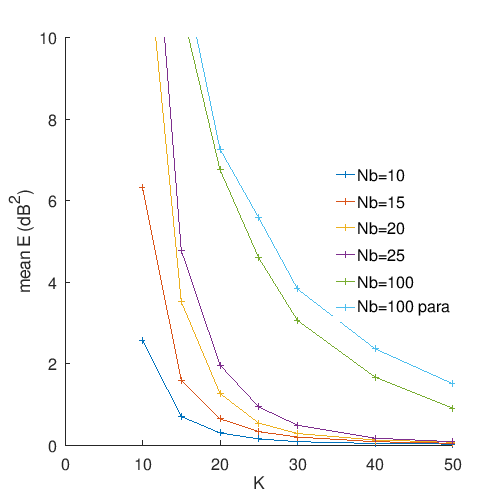
\includegraphics[width=10cm]{ratek2_E_K_hts.png}
\end{figure}


\end{document}

